\newpage
\section{Compiler Phases}
\label{sec:compiler_phases}

\begin{figure}[bth]
	\centering
	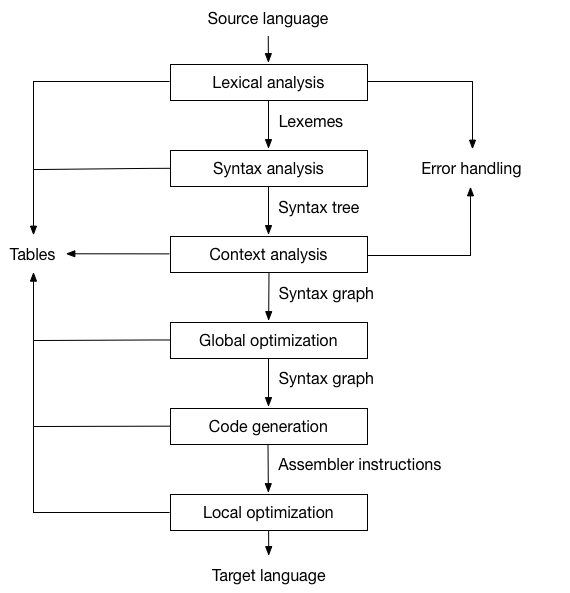
\includegraphics[scale=0.5]{./img/compiler_phases}
	\caption[Compiler phases]{Compiler phases}
	\label{fig:compiler_phases}
\end{figure}
\noindent

The figure \ref{fig:compiler_phases} shows the compilation process which starts with the input of a \emph{source program}. The program must be written in \emph{E}. 

The lexical, syntax and context analysis are a part of the analysis phase. This is primarily about the properties of the source program. The \emph{lexical analysis} is about recognizing words (see chapter \ref{sec:lexical_analysis} on page \pageref{sec:lexical_analysis}). The \emph{syntax analysis} then builds a logical structure of the lexemes (see chapter \ref{sec:syntactic_analysis} on page \pageref{sec:syntactic_analysis}). The \emph{context analysis}, on the other hand, includes e.g. a type test. The result is then a syntax graph. During these phases, \emph{errors} are always handled. Accordingly, the system checks, for example, whether a variable was used before the definition. The \emph{global optimization} makes an optimization on the source text. Thus e.g. isomorphies are summarized in the code.

The \emph{code generation} represents the synthesis. The structure of the source program already exists there. The synthesis consists of three components: 
\begin{itemize}
	\item \textbf{Allocation}: The available components like a Graphics Processing Unit (GPU) are selected.
	\item \textbf{Binding}: The specific functions are mapped to the components.
	\item \textbf{Control flow}: The chronological sequence of the commands is displayed.
\end{itemize}
It generates assembler instructions and is therefore dependent on the respective instruction set of the processor. This refers, for example, to the allocation of registers which is generally NP complete \cite{bdr2006}, i.e. there are only runtime-intensive algorithms for an exact solution. Moreover, hashtables are used for quick access to identifiers or strings. \emph{Local optimization} is again based on basic blocks. These start with the entry into a control flow and end with the exit. However, they do not include jumps. More about this topic can be found in chapter \ref{sec:code_generation} on page \pageref{sec:code_generation}. The main goal here is to rearrange commands. The bytecode for the source language \emph{E} then results.

Altogether, there is a difference between runtime and compile time which is shown in the tombstone diagram\footnote{Tombstone diagram, \url{http://www.informatik.uni-bremen.de/agbkb/lehre/uebersetzer/Kopien/BootstrapWatt.pdf}} \ref{fig:compile_time_runtime}:

\begin{figure}[bth]
	\centering
	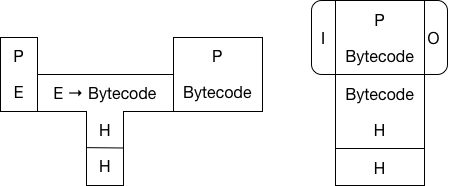
\includegraphics[scale=0.5]{./img/compile_time_runtime}
	\caption[Compile time and runtime]{Compile time and runtime}
	\label{fig:compile_time_runtime}
\end{figure}
\noindent

The compile time refers to the compiler phases (see figure \ref{fig:compiler_phases} on page \pageref{fig:compiler_phases}). The language \emph{E} is transformed by a host (H) to bytecode. The execution also happens there. The bytecode can then be interpreted at runtime where it is located in the Java Virtual Machine (JVM). Therefore it is also possible to generate code for different central processing units (CPU) like PowerPC or x86. However, the code can also be translated on a different architecture and then executed elsewhere. Accordingly, retargeting and rehosting are supported.

In the following, the respective components of the compiler will be explained. The following folder structure regarding the architecture is used as help:

\begin{verbatim}
e
   io
   ...
   std
   ...
   test
      main.e
grammar
   E.g4
lib
   antlr.jar
   jasmin.jar
src
   main
      java
         com
            runekrauss
               compiler
                  CustomType.java
                  CustomTypeVisitor.java
                  DataType.java
                  DataTypeStack.java
                  EVisitor.java
                  FunctionDefinitionVisitor.java
                  FunktionPrototype.java
                  FunctionPrototypeList.java
                  Main.java
                  StaticVariableVisitor.java
                  TypeInformation.java
                  exception
                     AlreadyDefinedFunctionException.java
                     ...
                     UndeclaredVariableException.java
                     ...
                     WrongDataTypeException.java
               parser
                  E.tokens
                  ...
                  EBaseVisitor.java
                  ELexer.java
                  EParser.java
                  EVisitor.java
      resources
         assembly
            inline_asm.e
            ...
         branch
         comments
         function
         loop
         operators
         ...
   test
      java
         com
            runekrauss
               compiler
                  CompilerTest.java
pom.xml
target
README.md
...
\end{verbatim}

The folder \emph{grammar} contains the defined grammar with the parser and lexer rules. In the folder \emph{lib} you can also find the used libraries for ANTLR and Jasmin (see chapter \ref{sec:code_generation} on page \pageref{sec:code_generation}). In summary, a Maven\footnote{Maven, \url{https://maven.apache.org}} project is used where these are listed as dependencies in the \emph{pom.xml} (see appendix on page \pageref{sec:maven}). The actual source files are divided into the folders \emph{compiler} and \emph{parser}. The \emph{compiler} folder contains the defined logic for traversing the tree with code generation (see chapter \ref{sec:context_analysis} on page \pageref{sec:context_analysis}) and the start method for starting a file such as \emph{main.e} written in the language \emph{E}. The folder \emph{e} also contains the standard library of the language that can be imported. The \emph{exception} package contains error classes for incorrect use of the described constructs regarding the context analysis of language \emph{E}. For example, a message is generated when a variable is used although it has not yet been declared. Another example would be that an error message appears when a function is defined twice or if a data type is not compatible with an operation. In the \emph{parser} folder there is a lexer and a parser to make analyses. The recognized tokens can also be found there. The unit and integrations tests can be found in the \emph{test} folder (see chapter \ref{sec:tests} on page \pageref{sec:tests}). The respective tests also read test files from the \emph{resources} folder if the corresponding source code is relatively long. Among other things, this refers to the tests for functions, branches, loops and operators. The respective compilates are created in the \emph{target} folder.

\textbf{Note}: For a better overview, several comments have been removed in the codes. However, these are visible in the \emph{E Compiler}\footnote{E Compiler, \url{https://github.com/RuneKrauss/eCompiler}} as a Maven project. The current description of the installation of the compiler is shown in the respective \emph{README.md}.

\subsection{Lexical analysis}
\label{sec:lexical_analysis}

Generally speaking, lexical analysis creates lexemes from source code. The scanner is responsible for recognizing lexemes. The screener, on the other hand, performs actions after recognition. This includes e.g. removing comments. Each lexeme consists of one or more characters. These include, for example, printable characters such as letters or numbers but also control characters such as tab stops. The encoding of the characters is limited to American Standard Code for Information Interchange (ASCII). The code can be found in the appendix on page \pageref{sec:ascii}.

The lexical analysis is done with finite automata, i.e. the lexemes are described by regular expressions.

\begin{defi}[Deterministic finite automaton]
	A deterministic finite automaton (DFA) is a 5-tuple, $(Q, \Sigma, \delta, q_0, F)$, consisting of a finite set of states $Q$, a finite set of input symbols called the alphabet $\Sigma$, a transition function $\delta : Q \times \Sigma \rightarrow Q$, an initial or start state $q_0 \in Q$ and a set of accept states $F \subseteq Q$.
\end{defi}

\begin{defi}[Nondeterministic finite automaton]
	A nondeterministic finite automaton (NFA) is represented by a 5-tuple, $(Q, \Sigma, \Delta, q_0, F)$, consisting of a finite set of states $Q$, a finite set of input symbols $\Sigma$, a transition relation $\Delta : Q \times \Sigma \rightarrow P(Q)$, an initial state $q_0 \in Q$ and a set of states $F$ distinguished as accepting or final states $F \subseteq Q$. Here, $P(Q)$ denotes the power set of $Q$.
\end{defi}

\begin{defi}[Regular expression]
	Be $\Sigma$ an alphabet. $\emptyset$ and $\epsilon$ are regular expressions, $a$ is a regular expression of $\Sigma$ for all $a \in \Sigma$. If $R_1$ and $R_2$ are regular expressions, then also $R_1 \cup R_2$, $R_1 \circ R_2$ and $R_1^*$ are regular expressions.
\end{defi}

\begin{defi}[Regular language]
	A regular language is a language that can be expressed with a regular expression or a deterministic or non-deterministic finite automata or state machine.
\end{defi}

\begin{defi}[Grammar]
	A grammar is a 4-tuple, $(N, \Sigma, P, S)$, consisting of a finite set $N$ of nonterminal symbols, a finite set $\Sigma$ of terminal symbols, a finite set $P$ of production rules with $(\Sigma \cup N)^* N(\Sigma \cup N)^* \rightarrow (\Sigma \cup N)^*$ and a distinguished symbol $S \in N$ that is the start symbol.
\end{defi}

Type-3 grammars generate regular languages and have a single non-terminal on the left-hand side as well as a right-hand side consisting of a single terminal or single terminal followed by a single non-terminal. The productions have the form $X \rightarrow a$ or $X \rightarrow aY$ where $X, Y \in N$ and $a \in \Sigma$. Moreover, the rule $S \rightarrow \epsilon$ is allowed if $S$ does not appear on the right side of any rule.

For the language \emph{E} there are different lexemes which can be distinguished as follows in code \ref{lst:le}:

\lstset{
	numbers=left,
	stepnumber=1,
	numbersep=5pt,
	numberstyle=\small\color{black},
	basicstyle=\ttfamily,
	keywordstyle=\color{black},
	commentstyle=\color{black},
	stringstyle=\color{black},
	frame=single,
	tabsize=2,
	caption=Implementation of grammar E}

\begin{lstlisting}[frame=htrbl, caption={Lexer rules of grammar {\ttfamily E}}, label={lst:le}, basicstyle=\scriptsize]
// ----------------------------------------------------------------------------------
// Here are the built-in functions of the language E where an access is possible even
// without imports.

BUILTINFUNCTION             : 'toInt'
                            | 'toFloat'
                            | 'toString'
                            | 'append'
                            | 'length'
                            ;

// ----------------------------------------------------------------------------------
// Represents the two truth values of logic (true, false).

BOOL                        : 'true'
                            | 'false'
                            ;

// ----------------------------------------------------------------------------------
// Refers to integers

INTEGER                     : (DIGIT)+
                            ;

// ----------------------------------------------------------------------------------
// Refers to floating point numbers

FLOAT                       : INTEGER DOT INTEGER
                            | DOT INTEGER
                            ;

// ----------------------------------------------------------------------------------
// Any number of characters, but as little as possible that the rule is still 
// fulfilled

STRING                      : QMARK .*? QMARK
                            ;

// ----------------------------------------------------------------------------------
// Identifiers

IDENTIFIER                  : LETTER(LETTER | DIGIT)*
                            ;

// ----------------------------------------------------------------------------------
// (Multi)line comments (but as little as possible that the rule is still fulfilled)

COMMENT                     : ('//' ~[\r\n]* '\r'? '\n' | '/*' .*? '*/' | '/**' 
                              .*? '*/') -> skip
;

// ----------------------------------------------------------------------------------
// Ignore control characters (the screener removes these)

WHITESPACE                  : [ \t\n\r]+ -> skip
                            ;

// ----------------------------------------------------------------------------------
// Here are the repeating tokens in the grammar

SCOLON                      : ';'
                            ;

DOT                         : '.'
                            ;

COMMA                       : ','
                            ;

ASSIGN                      : '='
                            ;

QMARK                       : '"'
                            ;

OPAREN                      : '('
                            ;

CPAREN                      : ')'
                            ;

OBRACE                      : '{'
                            ;

CBRACE                      : '}'
                            ;

OBRACKET                    : '['
                            ;

CBRACKET                    : ']'
                            ;

OCBRACKET                   : '[]'
                            ;

// ----------------------------------------------------------------------------------
// Letters (will never be counted as a token)

fragment LETTER             : [a-zA-Z_]
                            ;

// ----------------------------------------------------------------------------------
// Digits (used for data types and identifiers)

fragment DIGIT              : [0-9]
                            ;
\end{lstlisting}

Conventionally, the rules for the Lexer are written in capital letters. A distinction is also made between meta and object characters. Thus, for example \texttt{+} is a metacharacter which states that an integer must consist of at least one digit. However, \texttt{'toInt'} is an object character that defines a built-in function. Repeating tokens such as brackets \texttt{\{} etc. are stored separately. The different comments are removed by the screener. In addition, there are different data types:

\begin{itemize}
	\item Booleans like \texttt{true}
	\item Integers like \texttt{5}
	\item Floating point numbers like \texttt{0.5} or \texttt{.5}
	\item Strings like \texttt{"world"}
	\item Arrays
	\item Structures and the corresponding objects
\end{itemize}

The concrete composition of the arrays and structures can be seen in chapter \ref{sec:syntactic_analysis} on page \pageref{sec:syntactic_analysis}. A data type can be primitive or an object associated with references whereby they consist of fragments such as digits. A fragment will never be counted as a token, it only serves to simplify a grammar and makes the grammar more readable as well as easier to maintain. A special feature of the strings is that they may consist of any number of characters but only so few that the rule is still fulfilled. This ensures that strings may not apply beyond quotation marks. The same principle applies to comments. The keywords are still reserved. Furthermore, the layout is not ignored. For this reason, no lookahead is required for the automatons. Finally, the performance is increased.
In addition, the compiler also knows the position in the source code so that more concrete error messages can be output (see chapter \ref{sec:context_analysis} on page \pageref{sec:context_analysis}). The generation of the automatons or tables for the lexemes is shown in the following figure \ref{fig:lexical_analysis}:

\begin{figure}[bth]
	\centering
	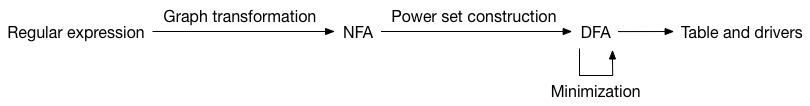
\includegraphics[scale=0.5]{./img/lexical_analysis}
	\caption[Workflow of the lexical analysis]{Workflow of the lexical analysis}
	\label{fig:lexical_analysis}
\end{figure}
\noindent

The workflow of the scanner is explained below using the example \texttt{R = LETTER(LETTER | DIGIT)*} (see figure \ref{fig:graph_transformation} on page \pageref{fig:graph_transformation}). First of all, the graph transformation takes place on the basis of rules. These come from the proof of the equivalence of finite automata and regular expressions \cite{v2013}. The rules for graph transformation can be found in the appendix on the page \pageref{sec:rules_graph_transformation}.

\begin{figure}[bth]
	\centering
	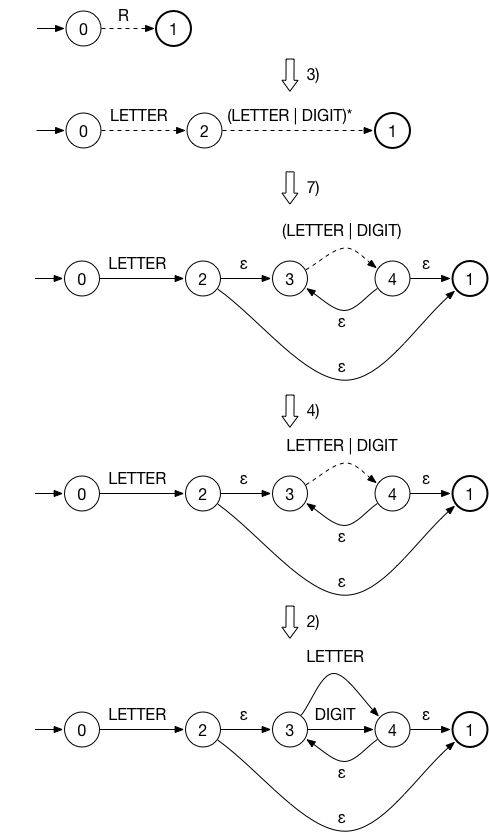
\includegraphics[scale=0.5]{./img/graph_transformation}
	\caption[Graph transformation on a regular expression]{Graph transformation on a regular expression}
	\label{fig:graph_transformation}
\end{figure}
\noindent

Accordingly, a NFA with epsilon transitions is formed. The epsilon transitions must then be removed and the powerset construction applied\footnote{Powerset construction, \url{http://www.cs.nuim.ie/~jpower/Courses/Previous/parsing/node9.html}}. First, states are marked for this purpose:

\newpage

\begin{figure}[bth]
	\centering
	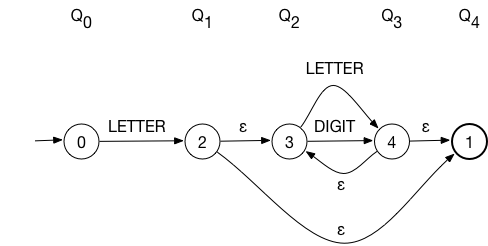
\includegraphics[scale=0.6]{./img/powerset_construction}
	\caption[Powerset construction at a NFA]{Powerset construction at a NFA}
	\label{fig:powerset_construction}
\end{figure}
\noindent

According to figure \ref{fig:powerset_construction}, the states $Q_0 = \{ 0 \}, Q_1 = \{ 2, 3, 1 \}, Q_2 = \{ 3 \}, Q_3 = \{ 4, 3, 1 \}$ are reached depending on the epsilon transitions. $Q_4$ is dropped here because there is nothing to read. Because the DFA states consist of sets of NFA states, an n-state NFA may be converted to a DFA with at most $2^n$ states. A converted DFA has exactly $2^n$ states, so giving an exponential time complexity. However, this runtime can be neglected since it is before the compile time.

When minimizing, the same states are combined or unattainable states are removed. Two states are equal if they have the same transitions. In concrete terms, equivalence classes are formed by applying the Table Filling method\footnote{Table Filling method, \url{http://pages.cs.wisc.edu/~shuchi/courses/520-S08/handouts/Lec7.pdf}}. The resulting minimum DFA is shown in the figure \ref{fig:dfa_after_minimization} below.

\begin{figure}[bth]
	\centering
	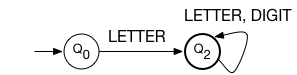
\includegraphics[scale=0.7]{./img/dfa_after_minimization}
	\caption[DFA after minimization]{DFA after minimization}
	\label{fig:dfa_after_minimization}
\end{figure}
\noindent

Afterwards, the DFA is mapped to a table \ref{tab:dfa_table}:

\begin{table}[bth]
	\centering
	\caption{Realization of a DFA in a table}
	\label{tab:dfa_table}
	\begin{tabular}{ | c | c | c | }
		\hline
		~ & \textbf{LETTER} & \textbf{DIGIT} \\ \hline
		0 & 2 & ~ \\ \hline
		2 & 2 & 2 \\ \hline
	\end{tabular}
\end{table}
\noindent

Valid words or identifiers are thus e.g. ``\_test'' or ``t3st''. Finally, all DFAs are combined for the respective lexemes. Alternatively, GOTO or WHILE programs\footnote{GOTO and WHILE programs, \url{https://www.informatik.hu-berlin.de/de/forschung/gebiete/algorithmenII/Lehre/ws11/einftheo/skript/einftheo-goto.pdf}} can be used instead of tables to show computability. The corresponding code can be found in the appendix on the page \pageref{sec:lexer}.

\subsection{Syntax analysis}
\label{sec:syntactic_analysis}

The syntax analysis generates an abstract syntax tree (AST) from lexeme sequences. The basis for this is the extended Backhus-Naur Form (EBNF) which is a metalanguage for the description of context-free or Type-2 grammars (CFGs). Type-2 grammars generate context-free languages. The productions must be in the form $X \rightarrow a$ where $X \in N$ and $a \in (\Sigma \cup N)^*$. These languages generated by these grammars are be recognized by a non-deterministic pushdown automaton.

\begin{defi}[BNF]
	The BNF is a formal notation for encoding grammars intended for human consumption. Every rule in BNF has the structure \texttt{name ::= expansion} where \texttt{::=} means ``may expand into'' and ``may be replaced with''. The \texttt{name} stands for a non-terminal symbol. Every name in BNF is surrounded by angle brackets, \texttt{<>} whether it appears on the left- or right-hand side of the rule. An expansion is an expression containing terminal and non-terminal symbols, joined together by sequencing and choice. A terminal symbol is a literal or a class of literals.
\end{defi}

\begin{defi}[EBNF]
	The EBNF is a collection of extensions to BNF but not all of these are strictly a superset, as some change the rule-definition relation \texttt{::=} to \texttt{=}, while others remove the angled brackets from non-terminals. Additional operations are options (\texttt{<term> ::= [ "-" ] <factor>}), repetitions (\texttt{<args> ::= <arg> { "," <arg> }}) and groupings (\texttt{<expr> ::= <term> ("+" | "-") <expr>}).
\end{defi}

In contrast to the conventional BNF, the EBNF therefore requires fewer constructs to describe CFGs. For example, options \texttt{[]} or repetitions \texttt{{}} can be used directly to present constructs more compactly instead of using recursions \cite{c2009}.

Essentially, a derivation tree is generated by the parser during the analysis which also states how it was derived. In this way, a differentiation was also made to a recognizer. As already mentioned in the introduction, ANTLR is used as a parser generator. ANTLR uses the top-down approach instead of a bottom-up parsing, i.e. a recursive descent parser is used. The input is processed from left to right by calculating a left derivation. This means that an attempt is made to create the desired word from a start symbol. Note that there are several language classes of CFGs that can be parsed deterministically whereby ANTLR handling $LL(k)$ grammars. The $k$ stands for the respective lookaheads that can be made. If there are many lookaheads, there are fewer conflicts but more states. At \emph{E} $k=1$ was set. The language classes are listed in the appendix on page \pageref{sec:det_cfg_classes}.

The parser is divided into three parts, a configuration, execution and actions which are explained in the following table \ref{tab:top_down_parsing}:

\begin{table}[bth]
	\centering
	\caption{Functionality of the recursive descent parser}
	\label{tab:top_down_parsing}
	\begin{tabular}{|l|l|}
		\hline
		\multicolumn{1}{|c|}{\textbf{Part}} & \multicolumn{1}{|c|}{\textbf{Description}} \\\hline
		Configuration                            & $\alpha . w$                                       \\\hline
		Execution                               & $s . w_0 \vdash^* \epsilon . \epsilon $                                       \\\hline
		Actions                                 & \makecell{\emph{match}: $a \alpha . aw \vdash_a \alpha . w$ \\ \emph{expand}: $A \alpha . w \vdash_p \beta \alpha . w$, where $p : A \rightarrow \beta \in P$}                                      \\\hline
	\end{tabular}
\end{table}

Here, $\alpha$ corresponds to the hypothesis $N^*$ and $w$ is the unread input. With regard to the execution, the start and end configuration are visible. The \emph{match} function is called when a terminal is derived. With \emph{expand}, on the other hand, a rule is generally applied. It is obvious that \emph{expand} as oracle advises the next application of a rule in doubt. If there is an error or a match, backtracking must be used and there is an exponential runtime. In order to obtain a linear runtime, special care was taken to define a deterministic CFG for the language \emph{E}. 

\begin{defi}[Ambiguous grammar]
	A grammar means ambiguous if $w \in \Sigma^*$ so that several derivation trees or left and right derivations exist.
\end{defi}

In general, it is undecidable whether a grammar is ambiguous which can be shown by a reduction of PKP to this problem \cite[p.461-462]{hmu2011}. In addition, a left factorization [$A \rightarrow \alpha \beta_1 \gamma, A \rightarrow \alpha \beta_2 \gamma$] $\rightarrow$ [$A \rightarrow \alpha B \gamma, B \rightarrow \beta_1, B \rightarrow \beta_2$] ($\alpha \neq \epsilon$) was used for the recursive descent regarding the processing. Thus, for example, precedents in arithmetic or logical operations are taken into account. In the following, the CFG for the language \emph{E} in code  \ref{lst:pe} is presented and explained:

\begin{lstlisting}[frame=htrbl, caption={Parser rules of grammar {\ttfamily E}}, label={lst:pe}, basicstyle=\scriptsize]
// Start rule
// It is evaluated from left to right.
// A program consists of statements, functions or structures.

program                     : incls+=includes* noMains+=noMain* command+ EOF
                            ;

// ----------------------------------------------------------------------------------
// Allows the import of different modules for e.g. mathematical calculations.

includes                    : 'use' OPAREN (mods+=module)+ (COMMA (mods+=module)*)*
                              CPAREN
                            ;

// ----------------------------------------------------------------------------------
// A namespace can consist of several modules that are separated from each other by 
// dots.

module                      : IDENTIFIER (DOT IDENTIFIER)*
                            ;

// ----------------------------------------------------------------------------------
// This indicates that no starting point is generated for a class.

noMain                      : '#define' name='noMain'
                            ;

// ----------------------------------------------------------------------------------
// This is a helper for the program because of functions and structs must not be in 
// the main method during code generation. Therefore statements, structs and 
// functions are separated.

command                     : statement #StatementCommand
                            | functionDefinition #FunctionDefinitionCommand
                            | structDeclaration #StructDeclarationCommand
                            ;

// ----------------------------------------------------------------------------------
// Statements in the program code (also without a semicolon at the end)
// Statements can stand alone and are not dependent on an expression.

statement                   : print SCOLON
                            | printLine SCOLON
                            | variableDeclaration SCOLON
                            | assignment SCOLON
                            | functionCall SCOLON
                            | branch
                            | loop
                            | includedFunctionCall SCOLON
                            | builtinFunctionCall SCOLON
                            | assembly
                            ;

// ----------------------------------------------------------------------------------
// Responsible for outputs without a new line

print                       : 'print' OPAREN arg=expression CPAREN
                            ;

// ----------------------------------------------------------------------------------
// Responsible for outputs with a new line

printLine                   : 'println' OPAREN arg=expression CPAREN
                            ;

// ----------------------------------------------------------------------------------
// Allows a declaration of variables (including an immediate initialization)

variableDeclaration         : type=dataType varId=IDENTIFIER (ASSIGN expr=expression)?
                            ;

// ----------------------------------------------------------------------------------
// Assigning values to a variable or struct

assignment                  : varId=IDENTIFIER ASSIGN expr=expression
                            | varId=IDENTIFIER OBRACKET index=expression CBRACKET 
                              ASSIGN expr=expression
                            | structVariableAssignment
                            ;

// ----------------------------------------------------------------------------------
// This can be used to assign values to structures.

structVariableAssignment    : structId=IDENTIFIER DOT varId=IDENTIFIER ASSIGN
                              expr=expression
                            | structId=IDENTIFIER DOT varId=IDENTIFIER OBRACKET
                              index=expression CBRACKET ASSIGN expr=expression
                            ;

// ----------------------------------------------------------------------------------
// Indicates a function call (with arguments).

functionCall                : funcId=IDENTIFIER OPAREN 
                              currentParams=currentParameters CPAREN
                            ;

// ----------------------------------------------------------------------------------
// Identifies a branch through which decisions can be made (else block is optional).

branch                      : 'if' OPAREN cond=expression CPAREN onTrue=block 
                              ('else' onFalse=block)?
                            ;

// ----------------------------------------------------------------------------------
// Realizes while loops whereby Turing-completeness applies.

loop                        : 'while' OPAREN cond=expression CPAREN body=block
                            ;

// ----------------------------------------------------------------------------------
// With this you can directly write assembler in high level language. Assembly can be
// executed or written directly. However, objects can also be initialized directly.

assembly                    : 'asm' OBRACE str=STRING CBRACE #InlineAssembly
                            | 'invoke' mod=STRING id=STRING OPAREN args+=jvmType* 
                              CPAREN returnType=STRING SCOLON #InvokeAssembly
                            | 'new' type=STRING SCOLON #InitObject
                            | 'pushToStack' expression SCOLON #PushToStack
                            | 'setTopOfStack' type=STRING SCOLON #SetTopOfStack
                            ;

// ----------------------------------------------------------------------------------
// The supported types of the JVM

jvmType                     : STRING
                            ;

// ----------------------------------------------------------------------------------
// This can be used to access functions from other packages.

includedFunctionCall        : inclDir=IDENTIFIER DOT funcId=IDENTIFIER OPAREN
                              args=currentParameters CPAREN ':' type=dataType
                            ;

// ----------------------------------------------------------------------------------
// Can be used to call built-in functions such as castings (without any imports).

builtinFunctionCall         : funcId=BUILTINFUNCTION OPAREN
                              currentParams=currentParameters CPAREN
                            ;

// ----------------------------------------------------------------------------------
// Definition of a function with parameters and a body with (several) statements 
// (a return value is optional)

functionDefinition          : type=dataType funcId=IDENTIFIER OPAREN
                              formalParams=formalParameters CPAREN OBRACE
                              stmts=statements ('return' returnVal=expression 
                              SCOLON)? CBRACE
                            ;

// ----------------------------------------------------------------------------------
// Describes the declaration of a structure with at least one variable.

structDeclaration           : 'struct' structId=IDENTIFIER OBRACE
                              (decls+=variableDeclaration SCOLON)+ CBRACE
                            ;

// ----------------------------------------------------------------------------------
// Initializes an object.

structArrayInitialization   : 'new' object=dataType OPAREN args=assignments CPAREN
                            | 'new' type=primitive OBRACKET size=expression CBRACKET
                            ;

// ----------------------------------------------------------------------------------
// Helper for initialization to assign values

assignments                 : asgmts+=expression (COMMA asgmts+=expression)*
                            ;

// ----------------------------------------------------------------------------------
// Mathematical operators
// Precedence (partial order): neg, (div, mul, rem), (sub, add), comp (same
// precedences), and, or, ... Labels allow access in the code.

expression                  : '-' expression #UnaryMinusExpression
                            | expression op=('/' | '*' | '%') expression
                              #DivisionMultiplicationModuloExpression
                            | expression op=('-' | '+') expression  
                              #SubtractionAdditionExpression
                            | expression op=('<<' | '>>') expression #ShiftExpression
                            | expression op=('<' | '<=' | '>' | '>=' | '==' | '!=')
                              expression #RelationalExpression
                            | lExpr=expression '&&' rExpr=expression
                              #ConjunctionExpression
                            | lExpr=expression '||' rExpr=expression
                              #DisjunctionExpression
                            | expression '^' expression #ContravalenceExpression
                            | varId=IDENTIFIER OBRACKET index=expression CBRACKET
                              #ArrayExpression
                            | structId=IDENTIFIER DOT varId=IDENTIFIER 
                              #StructExpression
                            | structId=IDENTIFIER DOT varId=IDENTIFIER OBRACKET
                              index=expression CBRACKET #StructArrayExpression
                            | structInitialization #StructInitializationExpression
                            | bool=BOOL #BoolExpression
                            | number=INTEGER #IntegerExpression
                            | number=FLOAT #FloatingPointExpression
                            | str=STRING #StringExpression
                            | varId=IDENTIFIER #VariableExpression
                            | builtinFunctionCall #BuiltinFunctionExpression
                            | functionCall #FunctionExpression
                            | includedFunctionCall #IncludedFunctionExpression
                            | 'topOfStack' #TopOfStack
                            ;

// ----------------------------------------------------------------------------------
// The current parameter list of functions can be of any length (no visitor).

currentParameters           : exprs+=expression (COMMA exprs+=expression)*
                            |
                            ;

// ----------------------------------------------------------------------------------
// Provides a basic block with an entry and exit from a control flow (no visitor).

block                       : OBRACE statements CBRACE
                            ;

// ----------------------------------------------------------------------------------
// Helper for more statements regarding blocks (no visitor)

statements                  : statement*
                            ;

// ----------------------------------------------------------------------------------
// The formal parameter list of functions can be of any length (no visitor).
// The number of parameters is also saved.

formalParameters            : decls+=variableDeclaration (COMMA
                              decls+=variableDeclaration)*
                            |
                            ;

// Represents the different data types (including lists and objects)

dataType                    : primitive(OCBRACKET)?
                            | IDENTIFIER(OCBRACKET)?
                            ;

// ----------------------------------------------------------------------------------
// The supported (primitive) types

primitive                   : 'bool'
                            | 'int'
                            | 'float'
                            | 'String'
                            | 'void'
                            ;
\end{lstlisting}

It should be mentioned that first as well as follow sets $F_i(N)$ and $F_o(N)$ were created to promote a left factorization which is why double entries are not allowed. The first set includes the start of a derivative of the variable in the grammar and the follow set the subsequent derivatives of the symbols that are possible or where the variable can be used. It applies, for example, $F_i(variableDeclaration) = \{ var \}$ and $F_o(variableDeclaration) = \{ '=', ';' \}$. Conventionally, the parser rules consist only of minuscules. The start symbol of the grammar is \texttt{program}. The evaluation takes place from left to right. In the grammar different constructs of the language \emph{E} are listed. A program consists of commands, i.e. statements, structures and functions. \texttt{EOF} means in this context that it definitely parses to the end of the file, even if errors occur before it. This results in a total output of all errors made. Statements must be in the main program or in blocks of functions or structures. They can also contain expressions or appear again in statements. An example is \texttt{if-else}. It may contain expressions, but may appear in a loop. Functions as well as structures are outside in this context. They are separated from the main program. This means that definitions and declarations can also be made after use. There are commands such as:

\begin{itemize}
	\item Imports like \texttt{use(e.io.reader)}
	\item Import calls like \texttt{String r = reader.read(): String;}
	\item Macro Instructions like \texttt{\#define noMain}
	\item Outputs like \texttt{print("world");}
	\item Variable declarations or assignments like \texttt{int a;} as well as \texttt{float a = 5.3;}
	\item Function definitions like \texttt{void foo(int a, int b) \{ print(a*b); \}}
	\item Function calls like \texttt{foo(7, 8);}
	\item Branches like \texttt{if (x) \{ a = 5; \} else \{ a = 7; \}}
	\item Loops like \texttt{int i = 0; while (i < 3) \{ println(i); i = i + 1; \}}
	\item Built-in functions like \texttt{toInt(3.7);}
	\item Inline assembler like \texttt{invoke "static" "java/lang/System/nanoTime"() "J";}
	\item Structures like \texttt{struct Point \{ int x; int y; \}}
	\item Struct initializations like \texttt{Point p = new Point(1, 2);}
	\item Arrays like \texttt{int[] a = new int[5];}
	\item Arithmetic operators like \texttt{a + b}
	\item Shift operators like \texttt{a >> b}
	\item Relational operators like \texttt{a <= b}
	\item Logical operators like \texttt{a \&\& b}	
\end{itemize}

The use of while loops make \emph{E} Turing complete \cite{z2018}. For this reason, it can be used to simulate any Turing machine. This means that this system is able to recognize or decide other data-manipulation rule sets. It is also possible, for example, to specify expressions such as multiplication or a number directly within the output. In order to increase readability, various labels such as \texttt{arg=expression} has been assigned to \texttt{print}. This makes it easier to access the respective expression such as a number or string by \texttt{arg} via the context within the visitor pattern during traversing (see chapter \ref{sec:context_analysis} on page \pageref{sec:context_analysis}). The parser rules therefore directly access the lexer rules. Labels were also awarded for a rule that allows several derivatives. An example of this is the subtraction or addition that has the label \texttt{\#SubtractionAdditionExpression}. Thus this rule can later be addressed directly by \texttt{visitSubtractionAdditionExpression} during traversing and also has its own context \texttt{SubtractionAdditionExpressionContext}. The same applies analogously to the other commands. Labels must not comply with the rules or be duplicated. The respective precedents are guaranteed by the order in which ANTLR4 follows sequentially. Different expressions can also be used in blocks such as branches. This allows statements to exist that do not have a semicolon at the end. In addition, symbols such as \texttt{+=} ensure that parameters can be counted which is particularly important for functions and later type analysis. Basically, functions are divided into call and definition by \texttt{functionDefinition} as well as \texttt{functionCall}. Functions are defined in the header and there does not have to be a declaration of variables. Furthermore, they can also be overloaded, i.e. the same name with different but arbitrarily long parameters is possible. The same principle applies to self-defined types such as structures.

The top-down parser uses a (simplified) abstract syntax to create the commands shown in the figure \ref{fig:abstract_syntax}:

\begin{figure}[bth]
	\centering
	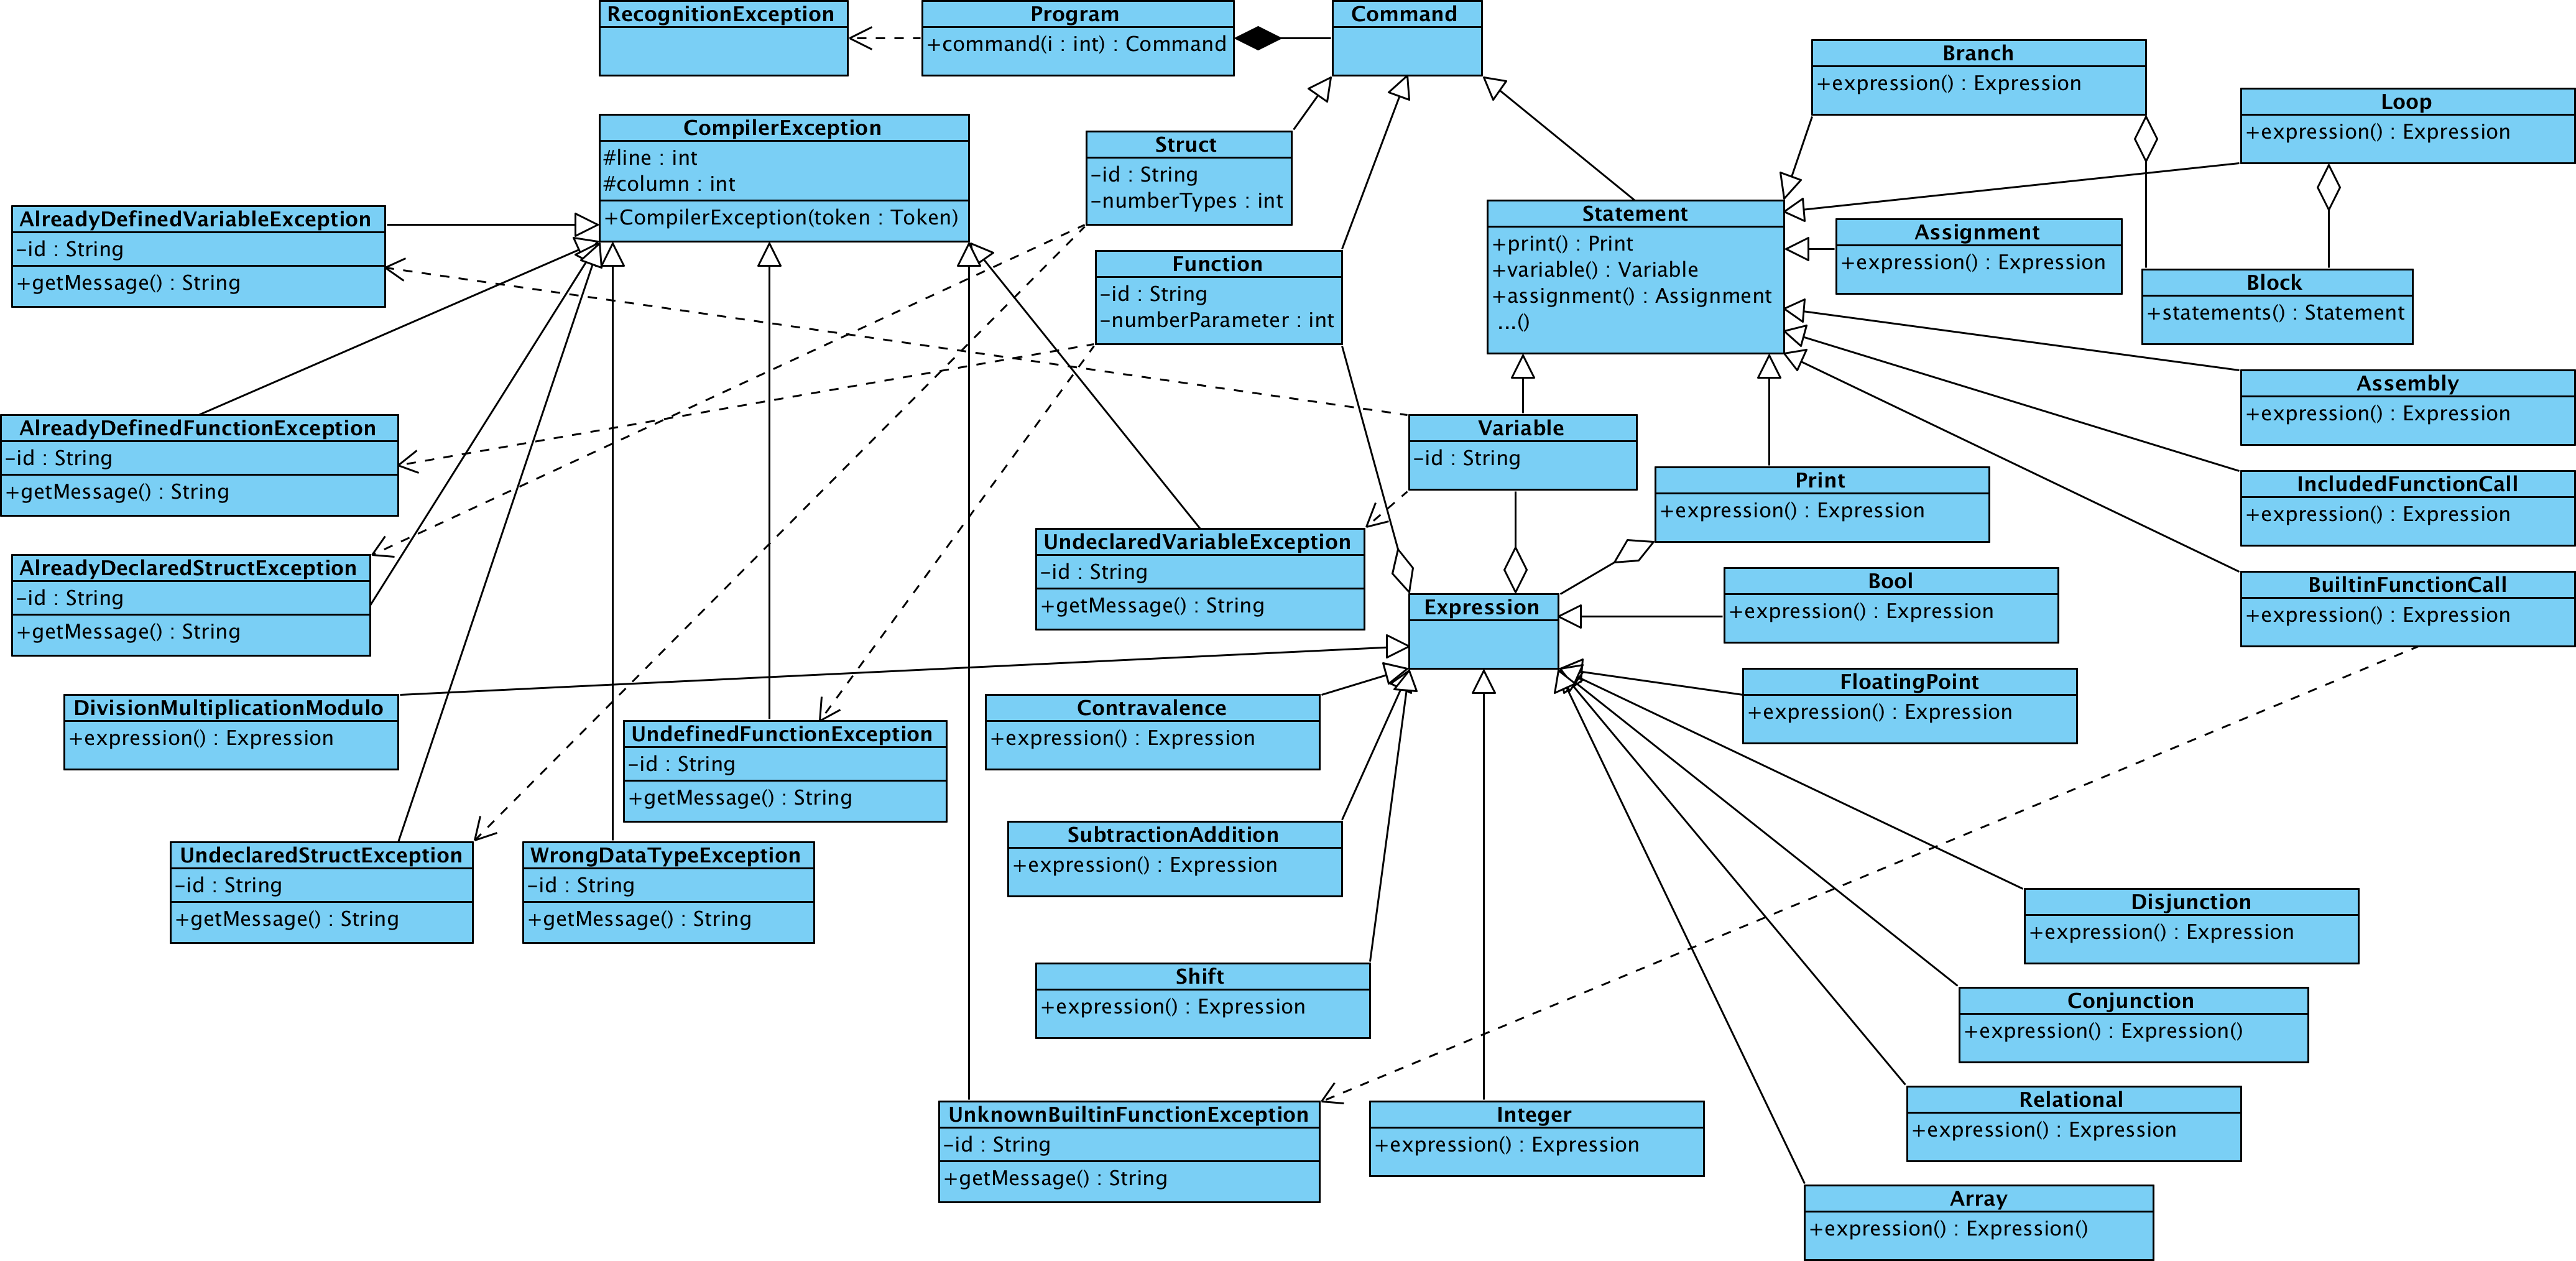
\includegraphics[scale=0.44]{./img/abstract_syntax}
	\caption[Abstract syntax]{Abstract syntax}
	\label{fig:abstract_syntax}
\end{figure}
\noindent

The AST is therefore described as an object structure by the abstract syntax. For simplicity, further edge markers, constructors and query functions have been omitted. Among other things, it can be recognized that commands cannot exist without a program. Furthermore, variables or functions can be used in expressions that are evaluated. Expressions can also be used, for example, in branches. Certain associated error classes ensure that users of language \emph{E} are notified of incorrect operation. The corresponding instructions for creation are in this document (simplified) parser and can be found in the appendix on page \pageref{sec:parser}. There is a procedure for each parser rule where the next lexeme $l$ is treated. Error handling is also performed during parsing. For example, the character \texttt{@} does not belong to any expression and in this case a \texttt{RecognitionException} would be thrown because this object character is not known. If a procedure is called, then $l \in F_i$ applies before. Then $l \in F_o$ is valid.

In the following, an AST is generated from the program code \texttt{print(3+2*4)} as an example:
\begin{align*}
program &\vdash command;\\
&\vdash statement;\\
&\vdash print;\\
&\vdash print(expression);\\
&\vdash print(expression\text{ }+\text{ }expression);\\
&\vdash print(3+expression);\\
&\vdash print(3+expression*expression);\\
&\vdash print(3+2*expression);\\
&\vdash print(3+2*4);
\end{align*}

Thus, a derivation tree could be successfully generated whereby the precedents are controlled by the ranking order. This also means that an ambiguous grammar must be checked. The corresponding AST is shown in figure \ref{fig:ast} on page \pageref{fig:ast}:

\newpage

\begin{figure}[bth]
	\centering
	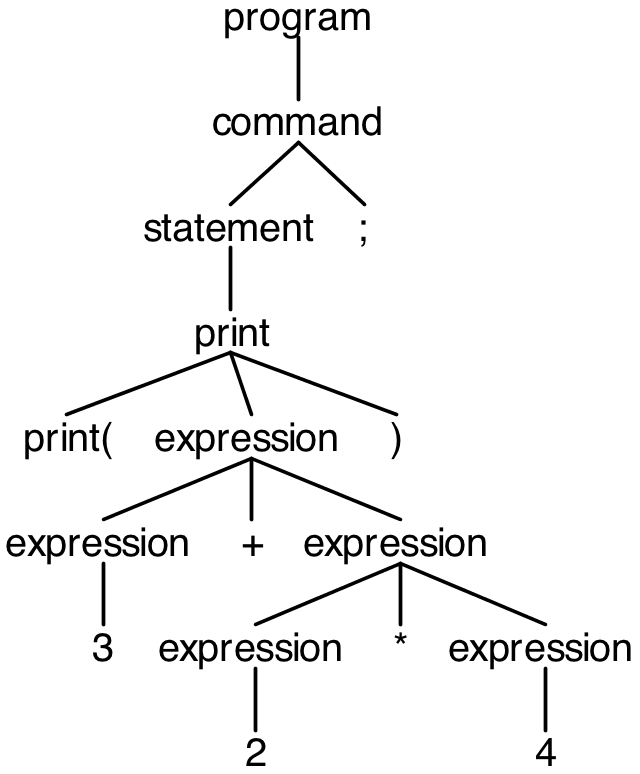
\includegraphics[scale=0.65]{./img/ast}
	\caption[Abstract syntax]{Abstract syntax tree}
	\label{fig:ast}
\end{figure}
\noindent

Due to the recursive definitions, a tree with theoretically infinite depth is created and can be traversed post-order to generate the instructions which will be explained in the next chapter.

\subsection{Context analysis}
\label{sec:context_analysis}

In general, an AST is marked with attributes during context analysis. These stand for cross-references with regard to definitions or usage. The AST then becomes an abstract syntax graph (ASG) which can also contain cycles due to recursions. The general steps are as follows:

\begin{enumerate}
	\item \textbf{Declaration analysis}: Checks, for example, whether a variable was declared before use.  
	\item \textbf{Type analysis}: Checks, for example, whether formal and current parameters match for functions.
\end{enumerate}

Thus, all rules that cannot be covered with a scanner (see chapter \ref{sec:lexical_analysis} on page \pageref{sec:lexical_analysis}) or parser must be checked. In the context, this includes both static (variable must have been defined) and dynamic conditions (a variable must be in the index area).

To describe the context conditions, a syntax-directed transduction is used instead of a two-level grammar, i.e. recursive functions are used on the AST.

On the described object structure from chapter \ref{sec:syntactic_analysis} on page \pageref{sec:syntactic_analysis} a general visitor can be defined who traverses the tree from which can be inherited later. A visit function is used to visit all connected elements. From this general visitor different visitors can be derived who define different operations on the AST. An excerpt of this visitor can be seen in the following code \ref{lst:visitor}:

\definecolor{javared}{rgb}{0.6,0,0} % Strings
\definecolor{javagreen}{rgb}{0.25,0.5,0.35} % Comments
\definecolor{javapurple}{rgb}{0.5,0,0.35} % Keywords
\definecolor{javadocblue}{rgb}{0.25,0.35,0.75} % Javadoc

\lstset{language=Java,
	basicstyle=\ttfamily,
	keywordstyle=\color{javapurple}\bfseries,
	stringstyle=\color{javared},
	commentstyle=\color{javagreen},
	morecomment=[s][\color{javadocblue}]{/**}{*/},
	numbers=left,
	numberstyle=\tiny\color{black},
	stepnumber=2,
	numbersep=10pt,
	tabsize=4,
	showspaces=false,
	showstringspaces=false}

\begin{lstlisting}[frame=htrbl, caption={Implementation of {\ttfamily EVisitor.java}}, label={lst:visitor}, basicstyle=\footnotesize]
public class EVisitor extends EBaseVisitor<String> {
   /** A list with all already defined functions */
   private final FunctionPrototypeList functions;

   /** Structs with declared variables and types (with references) */
   private final LinkedHashMap<String, CustomType> structs;

   /** Static variables in the main program (references to structs) */
   private final Map<String, TypeInformation> staticVarsNamesTypes;
...
   /** The namespace of the program you want to compile currently */
   private final String namespace;

   /** Descriptor for own declared types as reference */
   private final String typeNamespace;

   /** Parent directory (path to file for legacy) */
   private final File parentDir;

   /** Saves the module name as well as the path */
   private final Map<String, String> includedModules;

   /** Should a main method be created? */
   private boolean noMain;

   /** The variables in the table are accessed numerically. */
   private Map<String, TypeInformation> vars;

   /** Logs the used data types at compile time. */
   private DataTypeStack dataTypeStack;

   /** Is one in a function or the main program? */
   private boolean isGlobalScope;

   /** Counts the branches because no label may be ambiguous. */
   private int branchCounter;
...
   /** Needed when initializing a structure */
   private String lookupStoreCommand;

   /** Also required when initializing a structure */
   private String lookupLoadCommand;
   
   /** Holds the current id of a struct */
   private int lookupStructId;

   public EVisitor(FunctionPrototypeList definedFunctions, 
      LinkedHashMap<String, CustomType> declaredStructs, 
      Map<String, TypeInformation> declaredStaticVars, String namespace, 
      ...) {
      ...
   }

   @Override
   public String visitProgram(ProgramContext ctx) {
      // Generate potential code for the imports
      final int importNumber = ctx.incls.size();
      for (int i = 0; i < importNumber; ++i) {
         visit(ctx.getChild(i));
      }
      final int noMainNumber = ctx.noMains.size();
      for (int i = importNumber; i < noMainNumber; ++i) {
         visit(ctx.getChild(i));
      }
      final StringBuilder mainInstructions = new StringBuilder();
      final StringBuilder functionInstructions = new StringBuilder();
      // Regarding structs
      final StringBuilder extraClassesInstructions = new StringBuilder();
      for (int i = importNumber; i < ctx.getChildCount() - 1; ++i) {
         final ParseTree child = ctx.getChild(i);
         // Visit a parse tree and return a result of the operation
         final String instructions = visit(child);
         if (child instanceof StatementCommandContext) {
            mainInstructions.append(instructions).append('\n');
         } else if (child instanceof StructDeclarationCommandContext) {
            // The structures are marked accordingly because afterwards 
            // own files are created for them
            extraClassesInstructions.append("\n*").append(instructions)
               .append('\n');
         } else {
            functionInstructions.append(instructions).append('\n');
         }
      }
      final StringBuilder instructions = 
         new StringBuilder(".class public ")
         .append(namespace)
         .append("\n.super java/lang/Object\n\n")
         .append(staticVars.toString())
         .append('\n')
         .append(functionInstructions.toString())
         .append('\n');
      if (!noMain) {
         instructions
            .append(".method public static main([Ljava/lang/String;)V\n")
            .append(".limit stack ")
            .append(dataTypeStack.getMaxStackSize())
            .append("\n.limit locals 1\n\n")
            .append(mainInstructions.toString()).append("\nreturn\n\n")
            .append(".end method")
            .append(extraClassesInstructions.toString());
      } else {
         instructions.append(mainInstructions.toString()).append('\n')
            .append(extraClassesInstructions.toString());
      }
      return instructions.toString();
   }
...
   @Override
   public String visitIncludes(IncludesContext ctx) {
      for (int i = 0; i < ctx.mods.size(); ++i) {
         final String namespace = ctx.mods.get(i).getText()
            .replace('.', '_');
         final File file = new File(parentDir, namespace);
         final String address =
         file.getAbsolutePath().substring(parentDir
            .getAbsolutePath().length() + 1);
         if (!Main.programs.contains(address) &&
            !Main.compiledPrograms.contains(address)) {
            // Add the respective module to the compilation list
            Main.programs.add(address.replace("_", "/"));
         }
         final String fileName =
            file.getName().split("_")[file.getName()
               .split("_").length - 1];
         // Stores the filename ("math") and the path ("e_std_math") 
         // to the file (to compile)
         includedModules.put(fileName, address);
      }
      return "";
   }

   @Override
   public String visitPrint(PrintContext ctx) {
      final String argumentInstructions = visit(ctx.arg);
      // Get type to output
      final TypeInformation typeInfo = dataTypeStack.pop();
      // Get the associated JVM type
      String jvmType = typeInfo.getJvmType();
      if (typeInfo.getDataType() == DataType.OBJREF) {
         // Get the address (position) of the struct
         jvmType = 'L' + typeNamespace + jvmType + ';';
      }
      // Get the type that "visit" put on the stack
      return "getstatic java/lang/System/out Ljava/io/PrintStream;\n"
         + argumentInstructions
         + "\ninvokevirtual java/io/PrintStream/print("
         + jvmType + ")V\n";
   }
...
   @Override
   public String visitVariableDeclaration(VariableDeclarationContext 
      ctx) {
      String instructions = "";
      final Token varIdToken = ctx.varId;
      final String varId = varIdToken.getText();
      final String type = ctx.type.getText();
      // Get type object by type name
      final DataType dataType = DataType.getType(type);
      // Command to store a variable
      String storeCommand = "";
      final ExpressionContext exprContext = ctx.expr;
      if (isGlobalScope) {
         // When you are in the main method
         // Get type information by variable name
         final TypeInformation typeInfo = staticVarsNamesTypes
            .get(varId);
         lookupStoreCommand = "putstatic " + namespace + "/v" + typeInfo
            .getId();
         lookupLoadCommand = "getstatic " + namespace + "/v" + 
            typeInfo.getId();
         storeCommand = "putstatic " + namespace + "/v";
         // Descriptor for field access
         String descriptor;
         if (dataType == DataType.OBJREF) {
            descriptor = "L" + typeNamespace + structs.get(type)
               .getId() + ';';
            vars.put(varId, new TypeInformation(vars.size(), 
               dataType, structs.get(type).getId()));
         } else {
            descriptor = dataType.getJvmType();
            vars.put(varId, new TypeInformation(vars.size(), dataType));
         }
         staticVars.append(".field public static v")
            .append(getVariableIndexByVariableIdToken(varIdToken))
            .append(' ').append(descriptor).append('\n');
         if (exprContext != null) {
            instructions = visit(exprContext) + '\n' + storeCommand +
               getVariableIndexByVariableIdToken(varIdToken) + ' ' + 
               descriptor;
            if (dataTypeStack.peek().getDataType() != dataType) {
               throw new WrongDataTypeException(varIdToken);
            }
            dataTypeStack.pop();
            return instructions;
         }
         return instructions;
      } else {
         // When you are in a function
         if (vars.containsKey(varId)) {
            throw new AlreadyDeclaredVariableException(varIdToken);
         }
         if (dataType == DataType.OBJREF) {
            vars.put(varId, new TypeInformation(vars.size(), dataType,
               structs.get(type).getId()));
         } else {
            vars.put(varId, new TypeInformation(vars.size(), dataType));
         }
         final TypeInformation typeInformation = vars.get(varId);
         if (typeInformation.isArray() || dataType == DataType.STRING || 
            dataType == DataType.OBJREF) {
            storeCommand = "astore";
            lookupStoreCommand = storeCommand + ' ' + typeInformation
               .getId();
            lookupLoadCommand = "aload " + typeInformation.getId();
         } else if (dataType == DataType.INT) {
            storeCommand = "istore";
            lookupStoreCommand = storeCommand + ' ' + typeInformation
               .getId();
            lookupLoadCommand = "iload " + typeInformation.getId();
         } else if (dataType == DataType.FLOAT) {
            storeCommand = "fstore";
            lookupStoreCommand = storeCommand + ' ' + typeInformation
               .getId();
            lookupLoadCommand = "fload " + typeInformation.getId();
         }
         if (exprContext != null) {
            instructions = visit(exprContext) + '\n';
            instructions += storeCommand + ' ' +
                getVariableIndexByVariableIdToken(varIdToken);
            if (dataTypeStack.peek().getDataType() != dataType) {
               throw new WrongDataTypeException(varIdToken);
            }
            dataTypeStack.pop();
            return instructions;
         }
         return instructions;
      }
   }

   @Override
   public String visitAssignment(AssignmentContext ctx) { ... }

   @Override
   public String visitFunctionCall(FunctionCallContext ctx) { ... }

   @Override
   public String visitBranch(BranchContext ctx) { ... }
...
   @Override
   public String visitLoop(LoopContext ctx) { ... }

   @Override
   public String visitIncludedFunctionCall(IncludedFunctionCallContext 
      ctx) { ... }

   @Override
   public String visitBuiltinFunctionCall(BuiltinFunctionCallContext 
      ctx) { ... }

   @Override
   public String visitInlineAssembly(InlineAssemblyContext ctx) { ... }
...
   @Override
   public String visitFunctionDefinition(FunctionDefinitionContext 
      ctx) { ... }

   @Override
   public String visitStructDeclaration(StructDeclarationContext 
      ctx) { ... }

   @Override
   public String visitStructArrayInitialization(
      StructArrayInitializationContext ctx) { ... }
      
   @Override
   public String visitAssignments(AssignmentsContext ctx) { ... }

   @Override
   public String visitUnaryMinusExpression(UnaryMinusExpressionContext 
      ctx) { ... }

   @Override
   public String visitDivisionMultiplicationModuloExpression(
      DivisionMultiplicationModuloExpressionContext ctx) { ... }

   @Override
   public String visitSubtractionAdditionExpression(
      SubtractionAdditionExpressionContext ctx) { 
      String instructions = visitChildren(ctx);
      final TypeInformation typeInfo = dataTypeStack.peek();
      final DataType leftOperandType = dataTypeStack.pop().getDataType();
      final DataType rightOperandType = dataTypeStack.pop()
         .getDataType();
      // Only integer and floating point numbers are allowed
      if (leftOperandType != DataType.INT && leftOperandType != DataType
         .FLOAT || leftOperandType != rightOperandType) {
         throw new WrongDataTypeException(ctx.start);
      }
      final String arithmeticOperator = ctx.op.getText();
      switch (arithmeticOperator) {
         case "-":
            switch (typeInfo.getDataType()) {
               case INT:
                  instructions += "\nisub";
                  break;
               case FLOAT:
                  instructions += "\nfsub";
                  break;
               default:
                  throw new WrongDataTypeException(ctx.start);
            }
            break;
         case "+":
            switch (typeInfo.getDataType()) {
               case INT:
                  instructions += "\niadd";
                  break;
               case FLOAT:
                  instructions += "\nfadd";
                  break;
               default:
                  throw new WrongDataTypeException(ctx.start);
               }
               break;
         default:
            throw new IllegalArgumentException("Unknown arithmetic 
               operator: " + arithmeticOperator);
      }
      dataTypeStack.push(typeInfo);
      return instructions;  
   }

   @Override
   public String visitShiftExpression(ShiftExpressionContext ctx) { ... }

   @Override
   public String visitRelationalExpression(RelationalExpressionContext 
      ctx) { ... }

   @Override
   public String visitConjunctionExpression(ConjunctionExpressionContext 
      ctx) { ... }

   @Override
   public String visitDisjunctionExpression(DisjunctionExpressionContext 
      ctx) { ... }

   @Override
   public String visitContravalenceExpression(
      ContravalenceExpressionContext ctx) { ... }

   @Override 
   public String visitArrayExpression(ArrayExpressionContext ctx) { ... }

   @Override 
   public String visitStructExpression(StructExpressionContext 
      ctx) { ... }

   @Override 
   public String visitStructArrayExpression(StructArrayExpressionContext 
      ctx) { ... }

   @Override
   public String visitBoolExpression(BoolExpressionContext ctx) { ... }

   @Override
   public String visitIntegerExpression(IntegerExpressionContext 
      ctx) { 
      dataTypeStack.push(new TypeInformation(DataType.INT));
      return "ldc " + ctx.number.getText();
   }

   @Override
   public String visitFloatingPointExpression(
      FloatingPointExpressionContext ctx) { ... }


   @Override
   public String visitStringExpression(StringExpressionContext 
      ctx) { ... }

   @Override
   public String visitVariableExpression(VariableExpressionContext 
      ctx) { ... }
...
   @Override
   protected String aggregateResult(String aggregate, 
      String nextResult) {
      if (aggregate == null) {
         return nextResult;
      }
      if (nextResult == null) {
         return aggregate;
      } else {
      return aggregate + '\n' + nextResult;
   }
}
\end{lstlisting}

Accordingly, a semantic analysis can be realized in a visitor. Thus, new operations can be easily added by defining new visitors and related operations can be centrally managed in the visitor. The elements of the tree are visited which e.g. extends the symbol table information of variables. Expressions can also be checked to see if they are well typed. A visitor is used who also takes over the synthesis at the same time which will be explained in the next chapter.

To demonstrate how the tree is traversed, the example shall serve in the form of the figure \ref{fig:ast} on page \pageref{fig:ast}. The tree is traversed post-order due to the later code generation. Thus, the children are treated first before the parents are processed. Finally, the terminals are determined with \texttt{getText}. In the example, $3, 2, 4, *, +$ would be determined. As already mentioned, there is a corresponding method for each desired operation. Besides the methods of the base class for \texttt{program} and \texttt{statement}, \texttt{visitPrint} is called with the corresponding context. Then, \texttt{visit} is called with an expression as argument (here the addition) for producing the respective code. Now, \texttt{visitChildren} is called in \texttt{visitSubtractionAdditionExpression} where the context is passed. The method \texttt{visitChildren} visits the children of a node and returns a user-defined result of the specific operation. In contrast to this, the method \texttt{visit} visits a parse tree and return a user-defined result of the operation. On the one hand, \texttt{visitIntegerExpression} is called where the first number is determined. On the other hand, the right child is a multiplication where \texttt{visitDivisionMultiplicationModuloExpression} (analogous to addition) is called. Then, the further numbers are determined. Afterwards, the parents are determined, namely \texttt{*} and \texttt{+}. The corresponding aggregation of the string is explained in chapter \ref{sec:code_generation} on page \pageref{sec:code_generation}. Data types have also been implemented in the compiler. So only the integers and floating point numbers work in the arithmetic operations which is queried via conditions. Otherwise an exception is thrown. In order to manage the data types, a stack is used as data structure which is visible in code \ref{lst:dataTypeStack}:

\begin{lstlisting}[frame=htrbl, caption={Implementation of {\ttfamily DataTypeStack.java}}, label={lst:dataTypeStack}, basicstyle=\footnotesize]
public class DataTypeStack {
   /** A linked list of types */
   private final Deque<TypeInformation> typesStack;

   /** Maximum stack size for variables and so on */
   private int maxStackSize;

   DataTypeStack() {
      typesStack = new LinkedList<>();
      maxStackSize = 0;
   }

   public final void push(TypeInformation type) {
      if (type.getDataType() != DataType.VOID) {
         typesStack.push(type);
      }
      if (typesStack.size() > maxStackSize) {
         ++maxStackSize;
      }
   }

   public final TypeInformation pop() {
      return typesStack.pop();
   }

   public final TypeInformation peek() {
      return typesStack.peek();
   }

   public final int getMaxStackSize() {
      return maxStackSize + 1;
   }
}
\end{lstlisting}

The stack manages overall type information whereby this class is visible in code \ref{lst:typeInfo}:

\begin{lstlisting}[frame=htrbl, caption={Implementation of {\ttfamily TypeInformation.java}}, label={lst:typeInfo}, basicstyle=\footnotesize]
public class TypeInformation {
   /** Id (the position in the symbol table regarding variables) */
   private int id;

   /** Type of the construct (function, variable, ...) */
   private final DataType dataType;

   /** Address of a type (structure) regarding references */
   private int address;
...
   public final String getJvmType() {
      if (dataType != DataType.OBJREF) {
         return dataType.getJvmType();
      } else {
         return Integer.toString(address);
      }
   }

   public final boolean isArray() {
      switch (dataType) {
         case IARRAY:
         case FARRAY:
         case SARRAY:
            return true;
         default:
            return false;
      }
   }
}
\end{lstlisting}

This class stores a type and also an address if, for example, a reference to a structure exists. Accordingly, a variable can later be assigned to a structure. A distinction is made between objects and primitive data types that are visible in code \ref{lst:dataType}:

\begin{lstlisting}[frame=htrbl, caption={Implementation of {\ttfamily DataType.java}}, label={lst:dataType}, basicstyle=\footnotesize]
public enum DataType {
   /** A specific type regarding the JVM and E. */
   BOOL("bool", "Z"),
   INT("int", "I"),
   IARRAY("int[]", "[I"),
   FLOAT("float", "F"),
   FARRAY("float[]", "[F"),
   STRING("String", "Ljava/lang/String;"),
   SARRAY("String[]", "[Ljava/lang/String;"),
   VOID("void", "V"),
   OBJREF("", "");

   /** Type in E */
   private final String type;

   /** Type in the JVM */
   private final String jvmType;
...
   public static DataType getType(final String type) {
      switch (type) {
         case "bool":
            return BOOL;
         case "int":
            return INT;
         case "int[]":
            return IARRAY;
...
         default:
            return OBJREF;
      }
   }
...
}
\end{lstlisting}

For example, if an integer is called, the corresponding data type \texttt{INT} is pushed onto the stack. With an addition, this procedure is repeated. The addition can then pop these two data types from the stack and make decisions according to the code generation. The data type for the result is then pushed onto the stack again so that \texttt{print} uses the correct data type for the output. The individual abbreviations stand for the data type in binary code and are explained in the next chapter.

As already mentioned, the symbol table can also be extended in the context of variables. So in case of a variable declaration like \texttt{int a} the method \texttt{visitVariableDeclaration} is called and the position as well as the type is saved to the identifier. If a reference exists, the corresponding address for the object is also saved. If the variable already exists for an assignment, the position is determined and the corresponding value is saved. Otherwise, the procedure is analogous to the declaration. Later, the value of the variable can be retrieved if \texttt{visitVariableExpression} is called during traversing. Such expressions can also occur in branches or loops with blocks where the evaluation then takes place in \texttt{visitBranch} or \texttt{visitLoop}. Since labels must be unique, a counter \texttt{branchCounter} respectively \texttt{loopCounter} is incremented accordingly.

The same principle is not applied to functions because a function may be called if the definition is further down in the program. For this reason, functions have their own visitor which first collects the signatures (name and parameter types of the functions) and pass them to the visitor from code \ref{lst:visitor} on page \pageref{lst:visitor}. This also ensures total visibility. As already mentioned, a function can also have a body of any length. So that local variables can also be used, there are different local and one global scope. For example, the corresponding realization is visible in the method \texttt{visitFunctionPrototypes} where a new reference to an own symbol table is made. The visitor for functions is shown in code \ref{lst:visitor2}:

\begin{lstlisting}[frame=htrbl, caption={Implementation of {\ttfamily FunctionDefinitionVisitor.java}}, label={lst:visitor2}, basicstyle=\footnotesize]
public class FunctionDefinitionVisitor {
   public static FunctionPrototypeList findFunctionPrototypes(
      final ParseTree tree) {
      // Remember all prototypes of defined functions
      final FunctionPrototypeList definedFunctionPrototypes = 
         new FunctionPrototypeList();
      // Notice the built-in functions
      setBuiltInFunctionDefinitions(definedFunctionPrototypes);
      // An anonymous class
      new EBaseVisitor<Void>() {
         @Override
         public Void visitFunctionDefinition(FunctionDefinitionContext 
            ctx) {
            // Get return type
            final DataType returnType = DataType.getType(ctx.type
               .getText());
            // Get function identifier
            final String functionId = ctx.funcId.getText();
            final int paramNumber = ctx.formalParams.decls.size();
            final TypeInformation[] paramTypes = 
               new TypeInformation[paramNumber];
            // Get parameters
            for (int i = 0; i < paramNumber; ++i) {
               final DataType paramType =
                  DataType.getType(ctx.formalParams.decls.get(i)
                  .type.getText());
               if (paramType == DataType.VOID) {
                  throw new WrongDataTypeException(ctx.start);
               }
               paramTypes[i] = new TypeInformation(paramType);
            }
            // Has a function regarding the signature already been 
            // defined?
            if (definedFunctionPrototypes.contains(functionId, 
               paramTypes)) {
               throw new AlreadyDefinedFunctionException(ctx.funcId);
            }
            definedFunctionPrototypes.add(new 
               TypeInformation(returnType), functionId, paramTypes);
            return null;
         }
      }.visit(tree);
      return definedFunctionPrototypes;
   }
   
   private static void setBuiltInFunctionDefinitions(
      FunctionPrototypeList definedFunctions) {
      definedFunctions.add(new TypeInformation(DataType.VOID), "print", 
         new TypeInformation[] {new TypeInformation(DataType.INT)});
      ...
      definedFunctions.add(new TypeInformation(DataType.INT), "length",
         new TypeInformation[] {new TypeInformation(DataType.SARRAY)});
   }
}
\end{lstlisting}

Among other things, the built-in functions that a user can call later without importing are also defined here. In contrast to the main visitor, the implementation of \texttt{aggregateResult} is omitted. Thus states are omitted whereby the method for collecting the respective functions is pure which contributes to the increase of performance. This is stored in an additional list (see code \ref{lst:functionlist}):

\begin{lstlisting}[frame=htrbl, caption={Implementation of {\ttfamily FunctionPrototypeList.java}}, label={lst:functionlist}, basicstyle=\footnotesize]
public class FunctionPrototypeList {
   /** Contains all function prototypes from the respective program. */
   private final List<FunctionPrototype> functionPrototypes;
...
   public final boolean contains(final String functionId, final 
      TypeInformation[] params) {
      for (FunctionPrototype prototype : functionPrototypes) {
         // Get parameters of the current function in the list
         final TypeInformation[] functionParameters = prototype
            .getParams();
         // The function may only exist if the number of parameters and 
         // the function name match
         if (functionParameters.length == params.length &&  
            functionId.equals(prototype.getFunctionId())) {
            if (functionParameters.length == 0 && params.length == 0) {
               // There are no parameters available => 
               // The function signatures are the same
               return true;
            }
            boolean match = true;
            // Look more closely at the individual data types of 
            // the parameters
            for (int i = 0; i < functionParameters.length; ++i) {
               if (functionParameters[i].getDataType() != params[i]
                  .getDataType()) {
                  // Data types do not match => 
                  // function signatures cannot be the same
                  match = false;
                  break;
               }
            }
            if (match) {
               return true;
            }
         }
      }
      return false;
   }

   public final void add(final TypeInformation typeInfo, final String 
      functionId, final TypeInformation[] params) {
      functionPrototypes.add(new FunctionPrototype(typeInfo, functionId, 
         params));
   }
...
   public final FunctionPrototype get(final String functionId, final int 
      parameterNumber) {
      for (FunctionPrototype prototype : functionPrototypes) {
         if (prototype.getFunctionId().equals(functionId) && 
            prototype.getParamNumber() == parameterNumber) {
            return prototype;
         }
      }
      return null;
   }
}
\end{lstlisting}

The same principle also applies to structures that can be defined individually. There is also a separate visitor which first determines the names of the structures and maps them to positions. The following code \ref{lst:visitor3} shows this procedure:

\begin{lstlisting}[frame=htrbl, caption={Implementation of {\ttfamily CustomTypeVisitor.java}}, label={lst:visitor3}, basicstyle=\footnotesize]
public class CustomTypeVisitor {
   public static LinkedHashMap<String, CustomType> findTypes(final 
      ParseTree tree) {
      // Saves the names of the structures and their positions (from top 
      // to bottom).
      final Map<String, Integer> structIds = new LinkedHashMap<>();

      // Holds the structures with variables and types as well as 
      // references.
      final LinkedHashMap<String, CustomType> structs = 
         new LinkedHashMap<>();

      // An anonymous class (first round)
      new EBaseVisitor<Void>() {
         /** Position of the custom data type */
         int typeId = 0;

         @Override
         public Void visitStructDeclaration(StructDeclarationContext 
            ctx) {
            // The name of the structure must not appear twice
            if (structIds.get(ctx.structId.getText()) != null) {
               throw new AlreadyDeclaredStructException(ctx.structId);
            } else {
               structIds.put(ctx.structId.getText(), typeId++);
            }
            return null;
         }
      }.visit(tree);

      // An anonymous class (second round)
      new EBaseVisitor<Void>() {
         /** Position of the custom data type */
         int typeId = 0;

         @Override
         public Void visitStructDeclaration(StructDeclarationContext 
            ctx) {
            // Store the variables types
            final List<TypeInformation> varTypes = new ArrayList<>();
            // Maps the variable identifiers to its positions
            final Map<String, Integer> varIds = new HashMap<>();
            // Iterate over the variables in the structure
            for (int i = 0; i < ctx.decls.size(); ++i) {
               final String varType = ctx.decls.get(i).type.getText();
               // Get Data type object for the desired data type
               final DataType type = DataType.getType(varType);
               TypeInformation newType;
               if (type == DataType.OBJREF) {
                  final Integer structId = structIds.get(varType);
                  if (structId == null) {
                     throw new UndeclaredStructException(ctx.decls
                        .get(i).type.start);
                  } else {
                     // There is a reference => Map the variable type 
                     // to the struct position
                     newType = new TypeInformation(type, structId);
                  }
               } else {
                  newType = new TypeInformation(type);
               }
               varTypes.add(newType);
               final String varId = ctx.decls.get(i).varId.getText();
               if (!varIds.containsKey(varId)) {
                  varIds.put(varId, i);
               } else {
                  throw new AlreadyDeclaredVariableException(ctx.decls
                     .get(i).varId);
               }
            }
            structs.put(ctx.structId.getText(), new CustomType(typeId++, 
               varTypes, varIds));
            return null;
         }
      }.visit(tree);
      return structs;
   }
}
\end{lstlisting}

Then, references can also be determined within \texttt{visitStructDeclaration}. It is possible that types are defined in types which is why a double traversing occurs. Afterwards, the names of the types as well as the attributes and references are stored in a map. In the last traversing before the main traversing the static variables are determined which is shown in the following code \ref{lst:visitor4}:

\begin{lstlisting}[frame=htrbl, caption={Implementation of {\ttfamily StaticVariableVisitor.java}}, label={lst:visitor4}, basicstyle=\footnotesize]
public class StaticVariableVisitor {
   public static Map<String, TypeInformation> findStaticVariables(
      final ParseTree tree, final LinkedHashMap<String, CustomType> 
      structs) {
      // Saves the names and types (also references) of the static 
      // variables.
      final Map<String, TypeInformation> staticVars = new HashMap<>();

      // An anonymous class
      new EBaseVisitor<Void>() {
         int typeId = 0;

         @Override
         public Void visitProgram(ProgramContext ctx) {
            for (ParseTree child : ctx.children) {
               if (child instanceof StatementCommandContext) {
                  visit(child);
               }
            }
            return null;
         };

         @Override
         public Void visitVariableDeclaration(VariableDeclarationContext 
            ctx) {
            final String varType = ctx.type.getText();
            final DataType dataType = DataType.getType(ctx.type
               .getText());
            final String varId = ctx.varId.getText();
            if (staticVars.containsKey(varId)) {
               // A variable must not be declared twice
               throw new AlreadyDeclaredVariableException(ctx.varId);
            } else if (dataType == DataType.OBJREF) {
               final CustomType struct = structs.get(varType);
               if (struct == null) {
                  throw new UndeclaredStructException(ctx.start);
               } else {
                  // There is a reference => Map the variable type to  
                  // the struct position
                  staticVars.put(varId, new TypeInformation(typeId, 
                     dataType, struct.getId()));
               }
            } else {
               // Primitive data type
               staticVars.put(varId, new TypeInformation(typeId, 
                  dataType));
            }
            ++typeId;
            return null;
         }
      }.visit(tree);
      return staticVars;
   }
...
}
\end{lstlisting}

If there is a reference to a structure, the respective address including the type is inserted, otherwise only the data type. Later, a decision is made between a global or local scope (for functions) about the variable \texttt{isGlobal} which specific code is generated. So if, for example, the construct \emph{struct A \{ int a; \} A a = new A(0);} is present, then \texttt{Point 0 \{int, int\}} and \texttt{p : 0} would apply with regard to a debug mode, i.e. \texttt{p} refers to \texttt{Point}. In the case of further structures, the number would be increased. For example, the numbers are then used later during code generation as indexes for variables.

Due to the increased complexity there is an exception handling. In concrete terms, type and declaration analysis are implemented here in the form of exceptions for which a base class \ref{lst:exception} is used:

\begin{lstlisting}[frame=htrbl, caption={Implementation of {\ttfamily CompilerException.java}}, label={lst:exception}, basicstyle=\footnotesize]
public class CompilerException extends RuntimeException {

   protected int line;

   protected int column;

   public CompilerException(Token token) {
      line = token.getLine();
      column = token.getCharPositionInLine();
   }
}
\end{lstlisting}

If a construct of language \emph{E} is used incorrectly, the row, column and reason are specified within the traversal. For example, there are the following exceptions:

\begin{itemize}
	\item If a variable was not declared before use
	\item If a variable has been defined twice with respect to the identifier
	\item If a function was not defined before use
	\item If a function has been defined twice
	\item If a structure was not defined before use
	\item If a structure has been defined twice
	\item If a wrong data type was used inside an illegal operation
	\item If an unknown built-in function was used
	\item If an unknown imported module was used
\end{itemize}

\textbf{Note}: The exceptions refer to the specific scope.

In the case of \texttt{print(a);} the exception \texttt{1:6 <Undeclared variable: <a>;} is thrown into \texttt{visitVariableDeclaration} (see chapter \ref{sec:tests} on page \pageref{sec:tests}) if the identifier is not in the hash table. The same applies to variables that have already been defined. With regard to functions the signature decides whether a function is duplicated or not. As already mentioned, this check is already carried out in the \texttt{FunctionDefinitionVisitor} (see code \ref{lst:visitor2} on page \pageref{lst:visitor2}). If, for example, a \texttt{float get\_val() \{ return 1.0; \} float get\_val() \{ return 2.0; \}} was programmed, the message \texttt{2:4 Already defined function: <get\_val>;} would appear. The respective body and a correct function call are still checked in the main visitor (see code \ref{lst:visitor} on page \pageref{lst:visitor}). In addition, all operations are checked to see whether the data types are compatible with them. For example, if an attempt is made to call the code \texttt{String a = 5.0 + 3;}, a \texttt{WrongDataTypeException} is thrown. This procedure can also be transferred to the other application scenarios.

The corresponding derived classes can be found in the appendix on page \pageref{sec:exceptions}.

\subsection{Code generation}
\label{sec:code_generation}

During code generation, components of the grammar are transformed into code by required instructions, depending on the respective architecture. Here, \emph{Jasmin}\footnote{Jasmin, \url{https://cs.au.dk/~mis/dOvs/jvmspec/ref-Java.html}} is used as assembler for the JVM where bytecode is generated from assembler-like instructions. This can then be interpreted or executed in the JVM. The instructions are described in ASCII format. The basic structure is as follows (see Code \ref{lst:jasmin}):

\begin{lstlisting}[frame=htrbl, caption={Basic structure of {\ttfamily Jasmin}}, label={lst:jasmin}, basicstyle=\footnotesize]
.class public E
.super java/lang/Object
...
.method public static main([Ljava/lang/String;)V
   .limit stack 100
   .limit locals 100
...
   return
.end method;
\end{lstlisting}

Jasmin statements are comments, directives and instructions. A comment begins with a semi-colon and the assembler ignores everything after that to the end of line. Directives like \texttt{.super} begin with a period and are executed by the assembler rather than the JVM. An instruction can consists of a label, an operator (also called a mnemonic) and operands. For example, these can be arithmetic or logical. The \texttt{.super} construct indicates an inheritance in which the corresponding packages must also be specified. The \texttt{[L} command specifies an argument with an array of a certain type (also called the descriptor). The symbol \texttt{V} stands for no return (also called Void). The command \texttt{.limit} can be used to specify upper limits for e.g. the stack or local variables. In this case, the \texttt{return} construct determines the end of the main method. Before this are all instructions, such as outputs or variable declarations which are determined during traversing by the AST.

Altogether, the individual programs written in \emph{E} are processed in a queue and compiled individually as shown in the following code \ref{lst:main}:

\begin{lstlisting}[frame=htrbl, caption={Implementation of {\ttfamily Main.java}}, label={lst:main}, basicstyle=\footnotesize]
public class Main {
   /** Temporary directory for the compiled files */
   private static Path tempDir;

   /** Parent directory (path to file for legacy) */
   private static File parentDir;

   /** The namespace of the program you want to compile currently */
   private static String namespace;

   /** Holds the programs (including path) to compile. */
   public static Queue<String> programs;

   /** Holds the compiled programs (including path). */
   public static Queue<String> compiledPrograms;

   public static void main(String[] args) throws Exception {
      // Path to the main program
      final String fileName = "e/test/main";
      // Create a temporary directory for programs compiled later
      tempDir = createTempDir(fileName);
      parentDir = tempDir.toFile();
      programs = new LinkedList<>();
      // Add the program you want to compile
      programs.add(fileName);
      compiledPrograms = new LinkedList<>();
      // Process the programs
      while (!programs.isEmpty()) {
         final String program = programs.poll();
         compiledPrograms.add(program);
         // Set the namespace for later references
         namespace = program.replace('/', '_');
         // The current file to compile
         final File currentFile = new File(parentDir.getPath(), 
            namespace + ".e");
         final CharStream srcCode = CharStreams.fromFileName(program + 
            ".e");
...
         // Separate the main program from the structures
         final String[] compiledCode = compile(srcCode).split("\\*");
         if (!compiledCode[0].isEmpty()) {
            final ClassFile classFile = new ClassFile();
            classFile.readJasmin(new StringReader(compiledCode[0]), "", 
               false);
            final Path outputPath = tempDir.resolve(currentFile
               .getAbsolutePath().substring(0, currentFile
               .getAbsolutePath().length() - 2) + ".class");
            classFile.write(Files.newOutputStream(outputPath));
            final ClassFile[] extraFiles = new ClassFile[compiledCode
               .length - 1];
            // Create class files for the declared structs
            for (int i = 0; i < compiledCode.length - 1; ++i) {
               final ClassFile file = new ClassFile();
               extraFiles[i] = file;
               file.readJasmin(new StringReader(compiledCode[i + 1]), 
                  "", false);
               final Path newPath = tempDir.resolve(file.getClassName() 
                  + ".class");
               file.write(Files.newOutputStream(newPath));
            }
         }
      }
      // Run the compiled program
      final String result = runClass(tempDir, fileName.replace("/", "_"
         ));
      // Delete the created temporary directory
      deleteTempDir();
   }

   public static String compile(final CharStream sourceCode) {
      // Control characters are ignored
      ELexer lexer = new ELexer(sourceCode);
      CommonTokenStream tokens = new CommonTokenStream(lexer);
      EParser parser = new EParser(tokens);
      // Start rule
      ParseTree tree = parser.program();
      // Collect all function definitions (without body)
      FunctionPrototypeList definedFunctionPrototypes =
         FunctionDefinitionVisitor.findFunctionPrototypes(tree);
      // Collect all structs with declared variables and types
      // (including references)
      LinkedHashMap<String, CustomType> declaredStructs =
          CustomTypeVisitor.findTypes(tree);
      // Collect all static variables in the main program
      // (including references to structs)
      Map<String, TypeInformation> declaredStaticVars =
         StaticVariableVisitor.findStaticVariables(tree, 
         declaredStructs);
      // Create an assembler program for Jasmin based on instructions
      return new EVisitor(definedFunctionPrototypes, declaredStructs,
         declaredStaticVars, namespace, parentDir).visit(tree);
   }
...
   public static String runClass(final Path dir, final String className)
      throws Exception {
      final Process process =
      Runtime.getRuntime().exec(new String[] {"java", "-cp", dir
         .toString(), className});
      try (InputStream input = process.getInputStream()) {
         Scanner scanner = new Scanner(input);
         if (scanner.useDelimiter("\\A").hasNext()) {
            String result = scanner.useDelimiter("\\A").next();
            scanner.close();
            return result;
         }
         scanner.close();
         return null;
      }
   }
}
\end{lstlisting}

In general, the main procedure is as follows:

\begin{enumerate}
	\item The main program is added to the queue.
	\item As long as the queue is not empty, do the following:
	\begin{enumerate}
		\item Get the current file to compile from the queue.
		\item Convert the file to a namespace (for class names, references, etc.).
		\item Compile the file in several steps (see figure \ref{fig:compiler_phases} on page \pageref{fig:compiler_phases}).
		\item If there are structures, they are stored in separate class files.
	\end{enumerate}
\end{enumerate}

Since there can also be imports (see \texttt{visitIncludes} in code \ref{lst:visitor} on page \pageref{lst:visitor}), these are also processed in the queue. Finally, the compiled code can be executed.

After the described context analysis (see chapter \ref{sec:context_analysis} on page \pageref{sec:context_analysis}) of the example from the figure \ref{fig:ast} on page \pageref{fig:ast} the following code \ref{lst:jasmin2} would be generated:

\begin{lstlisting}[frame=htrbl, caption={Generated code of {\ttfamily \emph{E}}}, label={lst:jasmin2}, basicstyle=\footnotesize]
.class public e_test_main
.super java/lang/Object

.method public static main([Ljava/lang/String;)V
   .limit stack 4
   .limit locals 1

   getstatic java/lang/System/out Ljava/io/PrintStream;
   ldc 3
   ldc 2
   ldc 4
   imul
   iadd
   invokevirtual java/io/PrintStream/print(I)V

   return
.end method
\end{lstlisting}

To produce this code, a \texttt{StringBuilder} is used (see \texttt{visitProgram} in code \ref{lst:visitor} on page \pageref{lst:visitor}). This procedure saves the use of various objects and thus increases performance. The command \texttt{getstatic} places the object behind \texttt{System/Out} on the stack. Furthermore, the constants 3, 2 and 4 are placed one after the other on the stack. The command \texttt{imul} multiplies the two top elements 4 and 2 and puts the result back on the stack. This is then added to the 3 by \texttt{iadd}. This procedure is visualized as follows (see figure \ref{fig:stack}):

\begin{figure}[bth]
	\centering
	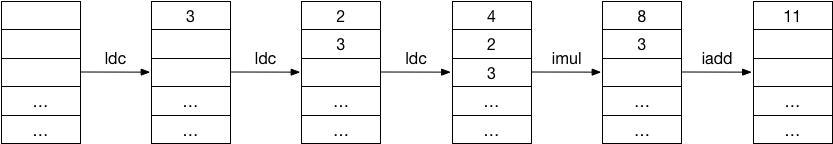
\includegraphics[scale=0.5]{./img/stack}
	\caption[Relation between the operations and stack]{Relation between the operations and stack}
	\label{fig:stack}
\end{figure}
\noindent

\textbf{Note}: If functions or structs are used, the respective parameters respectively attributes are also stored on the stack.

With the command \texttt{invokevirtual} the method \texttt{print} is called with an integer as argument which outputs the result. If the symbol table is to be extended with regard to variables, there are the commands \texttt{istore} and \texttt{iload} to store a value in a variable from the stack or to get a value from this position (see code \ref{lst:visitor} on page \pageref{lst:visitor}).

In addition, there are many other constructs such as branches, loops, different operators and so on. The following tables \ref{tab:trans}, \ref{tab:trans2} and \ref{tab:trans3} starting on page \pageref{tab:trans} show the transformation of various such constructs or examples:

\newpage

\begin{table}[bth!]
	\footnotesize
	\centering
	\caption{Code transformations}
	\label{tab:trans}
	\begin{tabular}{|l|l|l|}
		\hline
		\multicolumn{1}{|c|}{\textbf{Component}} & \multicolumn{1}{c|}{\textbf{Instructions}} & \multicolumn{1}{c|}{\textbf{Transformation}} \\ \hline		
		\makecell[l]{\texttt{void mul(int a} \\ \quad\texttt{,int b) \{} \\ \quad\texttt{print(a*b);} \\ \texttt{\}} \\ \texttt{mul(5, 3);}} & \makecell[l]{\texttt{getstatic} \\ \texttt{iload} \\ \texttt{imul} \\ \texttt{invokevirtual} \\ \texttt{ldc} \\ \texttt{invokestatic}} & \makecell[l]{\texttt{.method public static mul(II)V} \\ \texttt{.limit locals 2} \\ \texttt{.limit stack 3} \\ \texttt{getstatic java/lang/System/out Ljava/io/PrintStream;} \\ \texttt{iload 0} \\ \texttt{iload 1} \\ \texttt{imul} \\ \texttt{invokevirtual java/io/PrintStream/print(I)V} \\ \texttt{return} \\ \texttt{.end method} \\ \texttt{ldc 5} \\ \texttt{ldc 3} \\ \texttt{invokestatic e\_test\_main/mul(II)V}} \\ \hline	
		\makecell[l]{\texttt{int a = 1;} \\ \texttt{if (a) \{} \\ \quad\texttt{print(5);} \\ \texttt{\} else \{} \\ \quad\texttt{print(3);} \\ \texttt{\}}} & \makecell[l]{\texttt{ldc} \\ \texttt{putstatic} \\ \texttt{getstatic} \\ \texttt{ifne} \\ \texttt{goto}} & \makecell[l]{\texttt{ldc 1} \\ \texttt{putstatic main/v0 I} \\ \texttt{getstatic main/v0 I} \\ \texttt{ifne onTrue1} \\ \texttt{getstatic java/lang/System/out Ljava/io/PrintStream;} \\ \texttt{ldc 3} \\ \texttt{goto endIf1} \\ \texttt{onTrue1:} \\ \texttt{getstatic java/lang/System/out Ljava/io/PrintStream;} \\ \texttt{ldc 5} \\ \texttt{endIf1:}} \\ \hline
		\texttt{print(0 \&\& 1);} & \makecell[l]{\texttt{ldc} \\ \texttt{ifeq} \\ \texttt{goto} \\ \texttt{invokevirtual}} & \makecell[l]{\texttt{getstatic java/lang/System/out Ljava/io/PrintStream;} \\ \texttt{ldc 0} \\ \texttt{; jump if a is zero} \\ \texttt{ifeq onAndFalse1} \\ \texttt{ldc 0} \\ \texttt{ifeq onAndFalse1} \\ \texttt{ldc 1} \\ \texttt{goto endAnd1} \\ \texttt{onAndFalse1:} \\ \texttt{ldc 0} \\ \texttt{endAnd1:} \\ \texttt{invokevirtual java/io/PrintStream/print(I)V}} \\ \hline
	\end{tabular}
\end{table}
\noindent
With regard to the operations \texttt{and} and \texttt{or}, the direct use of the instructions \texttt{iand} and \texttt{ior} is deliberately waived in order to ensure lazy evaluation. With the disjunction the logic is only reversed in comparison to the conjunction. So that the labels for the jumps are unique, they are uniquely identified by a number.

\newpage

\begin{table}[bth]
	\footnotesize
	\centering
	\caption{Code transformations 2}
	\label{tab:trans2}
	\begin{tabular}{|l|l|l|}
		\hline
		\multicolumn{1}{|c|}{\textbf{Component}} & \multicolumn{1}{c|}{\textbf{Instructions}} & \multicolumn{1}{c|}{\textbf{Transformation}} \\ \hline
		\makecell[l]{\texttt{struct Point \{} \\ \quad\texttt{int x;} \\ \quad\texttt{int y;} \\ \texttt{\}} \\ \texttt{Point p = new} \\ \quad\texttt{Point(1, 2);} \\ \texttt{p.x = 5;}} & \makecell[l]{\texttt{aload} \\ \texttt{invokespecial} \\ \texttt{return} \\ \texttt{new} \\ \texttt{dup} \\ \texttt{putstatic} \\ \texttt{getstatic} \\ \texttt{putfield} \\ \texttt{ldc}} & \makecell[l]{\texttt{.class struct\_main0} \\ \texttt{.super java/lang/Object} \\ \texttt{.field public a0 I} \\ \texttt{.field public a1 I} \\ \texttt{.method public <init>()V} \\ \texttt{aload\_0} \\ \texttt{invokespecial java/lang/Object/<init>()V} \\ \texttt{return} \\ \texttt{.end method} \\ \texttt{} \\ \texttt{.class public main} \\ \texttt{.super java/lang/Object} \\ \texttt{.field public static v0 Lstruct\_main0;} \\ \texttt{.method public static main([Ljava/lang/String;)V} \\ \texttt{.limit stack 4} \\ \texttt{.limit locals 1} \\ \texttt{new struct\_main0} \\ \texttt{dup} \\ \texttt{invokespecial struct\_main0/<init>()V} \\ \texttt{putstatic main/v0 Lstruct\_main0;} \\ \texttt{getstatic main/v0 Lstruct\_main0;} \\ \texttt{ldc 1} \\ \texttt{putfield struct\_main0/a0 I} \\ \texttt{getstatic main/v0 Lstruct\_main0;} \\ \texttt{ldc 2} \\ \texttt{putfield struct\_main0/a1 I} \\ \texttt{getstatic main/v0 Lstruct\_main0;} \\ \texttt{putstatic main/v0 Lstruct\_main0;} \\ \texttt{getstatic main/v0 Lstruct\_main0;} \\ \texttt{ldc 5} \\ \texttt{putfield struct\_main0/a0 I} \\ \texttt{return} \\ \texttt{.end method}} \\ \hline
\end{tabular}
\end{table}
\noindent

A separate class is created for each structure. Attributes are assigned via \texttt{.field} and there is a default constructor that is initially loaded. In the main class there is a reference to this structure which is identified by \texttt{L}. A structure is created with \texttt{new} or the standard constructor is called with \texttt{invokespecial}. With \texttt{.putfield} values are assigned to the attributes. The suffixes of each variable name result from the position in the symbol table.

\newpage

\begin{table}[bth]
	\footnotesize
	\centering
	\caption{Code transformations 3}
	\label{tab:trans3}
	\begin{tabular}{|l|l|l|}
		\hline
		\multicolumn{1}{|c|}{\textbf{Component}} & \multicolumn{1}{c|}{\textbf{Instructions}} & \multicolumn{1}{c|}{\textbf{Transformation}} \\ \hline	
		\makecell[l]{\texttt{int[] a =} \\ \texttt{new int[3];} \\ \texttt{a[0] = 5;} \\ \texttt{print(a[0]);}} & \makecell[l]{\texttt{ldc} \\ \texttt{newarray} \\ \texttt{putstatic} \\ \texttt{getstatic} \\ \texttt{iastore} \\ \texttt{iaload} \\ \texttt{invokevirtual}} & \makecell[l]{\texttt{ldc 3} \\ \texttt{newarray int} \\ \texttt{putstatic main/v0 [I} \\ \texttt{getstatic main/v0 [I} \\ \texttt{ldc 0} \\ \texttt{ldc 5} \\ \texttt{iastore} \\ \texttt{getstatic java/lang/System/out Ljava/io/PrintStream;} \\ \texttt{getstatic main/v0 [I} \\ \texttt{ldc 0} \\ \texttt{iaload} \\ \texttt{invokevirtual java/io/PrintStream/print(I)V}} \\ \hline
			
		\makecell[l]{\texttt{int i = 0;} \\ \texttt{while (i < 3)} \\ \texttt{\{} \\ \quad\texttt{i = i + 1;} \\ \texttt{\}}} & \makecell[l]{\texttt{ldc} \\ \texttt{putstatic} \\ \texttt{getstatic} \\ \texttt{if\_icmplt} \\ \texttt{goto} \\ \texttt{ifeq} \\ \texttt{iadd}} & \makecell[l]{\texttt{ldc 0} \\ \texttt{putstatic main/v0 I} \\ \texttt{beginLoop1:} \\ \texttt{getstatic main/v0 I} \\ \texttt{ldc 3} \\ \texttt{if\_icmplt onCmpTrue1} \\ \texttt{ldc 0} \\ \texttt{goto endCmp1} \\ \texttt{onCmpTrue1:} \\ \texttt{ldc 1} \\ \texttt{endCmp1:} \\ \texttt{ifeq endLoop1} \\ \texttt{getstatic main/v0 I} \\ \texttt{ldc 1} \\ \texttt{iadd} \\ \texttt{putstatic main/v0 I} \\ \texttt{goto beginLoop1} \\ \texttt{endLoop1:}} \\ \hline
		\texttt{int i = 2 < 2;} & \makecell[l]{\texttt{ldc} \\ \texttt{if\_icmplt} \\ \texttt{goto} \\ \texttt{putstatic}} & \makecell[l]{\texttt{ldc 2} \\ \texttt{ldc 2} \\ \texttt{if\_icmplt onCmpTrue1} \\ \texttt{ldc 0} \\ \texttt{goto endCmp1} \\ \texttt{onCmpTrue1:} \\ \texttt{ldc 1} \\ \texttt{endCmp1:} \\ \texttt{putstatic main/v0 I}} \\ \hline
	\end{tabular}
\end{table}
\noindent

Overall, these results are aggregated. In code \ref{lst:visitor} on page \pageref{lst:visitor}, the method \texttt{visitChildren} can be recognized during traversing in this context. This method is executed on several nodes which is why the method \texttt{aggregateResult} is called internally there to aggregate the specific instructions. The relevant operands are also placed on the stack.

A list of more relevant commands with descriptions can be found in the appendix on page \pageref{sec:jasmin_instructions}. Finally, a more complex example can be found in the appendix on page \pageref{sec:eprogram}.